\documentclass[t]{beamer}
\usetheme{Boadilla} %\usetheme{Goettingen}
\usefonttheme{serif}
\usefonttheme{professionalfonts}
\usecolortheme{beaver}
\setbeamertemplate{itemize item}{•}
\setbeamertemplate{itemize subitem}{◦}
\setbeamertemplate{itemize subsubitem}{—}
\setbeamercolor*{itemize item}{fg=frametitle.fg}
\setbeamercolor*{itemize subitem}{fg=frametitle.fg}
\setbeamercolor*{itemize subsubitem}{fg=frametitle.fg}
\setbeamertemplate{section in toc}[default] % remove bullet from section on outline slide
\setbeamertemplate{subsection in toc}[default] % remove bullet from subsection on outline slide
\beamertemplatenavigationsymbolsempty % suppress navigation bar
\setbeamercovered{transparent=30} % global setting for slide builds (enabled by the <1-2> codes after \item)
\setbeamercolor{footnote mark}{fg=frametitle.fg}

\usepackage{fontspec, setspace, tabu, booktabs, multirow, url, calc}%, colortbl, etoolbox}
%\usepackage[shortcuts]{extdash}
%\usepackage[sort&compress,super]{natbib}
%\usepackage{dblfnote}
\usepackage{natbib}
% Use these with \footnotemark, \footnotetext & \bibentry if you want full references to show up on each slide
%\usepackage{bibentry} 
%\nobibliography*

% misc hacks
\def\newblock{\hskip .11em plus .33em minus .07em}
\definecolor{lgray}{gray}{0.7}
\definecolor{rdd}{HTML}{940013}
\definecolor{grn}{HTML}{005D00}
\definecolor{blu}{HTML}{004CBD}
\newcommand{\redd}[1]{{\bfseries\color{rdd}\ac{#1}}}
\newcommand{\grnn}[1]{{\bfseries\color{grn}\ac{#1}}}
\newcommand{\bluu}[1]{{\bfseries\color{blu}\ac{#1}}}
\newenvironment{hl}{\usebeamercolor[fg]{frametitle}}{}
\newenvironment{hid}{\usebeamercolor[bg]{background canvas}}{}

% fonts
\setmainfont[Numbers={Lining}]{Linux Libertine O} \setsansfont{Linux Biolinum O} \setmonofont{Linux Libertine Mono O}
\newfontfamily{\stix}{STIXGeneral-Regular}
%\newfontfamily{\charis}{Charis SIL}
%\newenvironment{ipa}{\large\charis}{}%
\renewcommand\url{\begingroup \def\UrlLeft{}\def\UrlRight{}\urlstyle{same}\Url} % set URLs in same font as surrounding text

% replacement for itemize environment
\newenvironment{itm}{%
	\setlength{\leftmargini}{0.5em}%
	\setlength{\leftmarginii}{1em}%
	\begin{itemize}}{\end{itemize}%
}

% misc abbreviations
\newcommand{\term}[1]{“#1”} % first occurrence of technical terms
\newcommand{\ac}[1]{\textsc{#1}} % acronyms % \newcommand{\ac}[1]{\MakeUppercase{#1}}
\newcommand{\lat}[1]{\textit{#1}} % foreign words and abbreviations
\newcommand{\psola}{\ac{psola}™}
\newcommand{\fo}{ƒ\kern-0.1em₀} % font problems? might work as {\(f_0\)}  
\newcommand{\eg}{\lat{e.g.}}
\newcommand{\ie}{\lat{i.e.}}
\newcommand{\etseq}{\lat{et seq}}
\newcommand{\etc}{\lat{etc}}
\newcommand{\intal}{\lat{inter alia}}
\newcommand{\ph}{\lat{post hoc}}
\newcommand{\Ph}{\lat{Post hoc}}
\newcommand{\aka}{\textsc{aka}}
\newcommand{\vs}{\lat{vs.}}
\newcommand{\vv}{\lat{vice versa}}
\newcommand{\perse}{\lat{per se}}
\newcommand{\slsh}{/\kern 1sp} % contains a zero-width non-joiner after the slash, to allow line breaking
%\newcommand{\slsh}{/‌} % contains a zero-width non-joiner after the slash, to allow line breaking
\newcommand{\refcomma}{{\hl\(^{\hspace{-0.1em},}\)}} % negative superscript space followed by superscript comma, in the highlight color (same color as the frametitle)

% formatting
\newenvironment{str}{\large\scshape\bfseries}{}%\textsf
\newcommand{\emp}[1]{{\hl\itshape #1}}
\newcommand{\fnr}[1]{\footnote[frame]{\citet*{#1}.}}
%\crefformat{footnote}{#2\footnotemark[#1]#3}
%\creflabelformat{footnote}{#2#1#3}

% Automatically insert overview/roadmap slide at start of each section
\AtBeginSection[]{%
\begin{frame}<beamer>
    \frametitle{Overview}
    \tableofcontents[currentsection,subsections,hideothersubsections] %\tableofcontents[currentsection]
  \end{frame}
}

\title[Prosody, intelligibility \& familiarity]{Prosody, intelligibility and familiarity\\in speech perception}
%\subtitle[short subtitle]{long subtitle}
\author[McCloy]{Daniel~McCloy} 
\institute[UW]{Department of Linguistics, University of Washington}
\date[2013.05.31]{2013 May 31}
\subject{Linguistics, Phonetics, Speech Perception}

\renewcommand*{\footnoterule}{}%\kern 6pt
\makeatletter
\renewcommand\@makefntext[1]{\leftskip=1em\hskip-1em{\tiny\@makefnmark~#1}}
%\patchcmd{\@makefntext}{\insertfootnotetext{#1}}{\insertfootnotetext{\tiny#1}}{}{} % requires etoolbox, achieves \tiny but has ugly first-line indenting
\makeatother

%\makeatletter
%\patchcmd{\@makefnmark}{\@textsuperscript}{\@makefnmark@aux}{}{}
%\newcommand*{\@makefnmark@aux}[1]{[#1]}
%makeatother
%\setbeamertemplate{footnote}{%
%    \leavevmode \insertfootnotemark~\insertfootnotetext
%}

\begin{document}

%===== TITLEPAGE =====%
\frame{\titlepage}


%===== TABLE OF CONTENTS =====%
\begin{frame}{Overview}
    \tableofcontents[section,hidesubsections]{}
%	\tableofcontents{}
\end{frame}


%===== DEFINITIONS =====%
\section{Definitions}

\subsection{Intelligibility}
\begin{frame}{Definition of intelligibility}
	\begin{itm}
	\item[] Intelligibility: degree to which speech can be understood
		\begin{itm}
		\item[]
		\item Measured as perception of words, not comprehension of meaning
		\item[]
		\item Usually speech-in-noise or degraded speech
%		\item[]
%		\item “Repeat what you hear” or “which word was it” tasks
		\end{itm}
	\end{itm}
\end{frame}

\subsection{Prosody}
\begin{frame}{Definition of prosody}
	\begin{itm}
	\item[] Prosody: phrase- or utterance-level patterns of \fo, duration \& intensity%\\(cf. Wikipedia: “intonation, rhythm \& stress”)
		\begin{itm}
		\item[]
		\end{itm}
	\item<2-> \fo, duration \& intensity modulated at smaller time scales too:
		\begin{itm}
		\item Word level
			\begin{itm}
			\item stressed\slsh unstressed vowel duration, frequency\slsh neighborhood effects, \etc.
			\item[]
			\end{itm}
		\item Segmental level
			\begin{itm}
			\item “i\fo”, voiced obstruent pitch depression, duration as secondary voicing cue, intrinsic segmental intensity differences, \etc.
			\item[]
			\end{itm}
		\end{itm}
	\item<3> Phrase-level modulations in \fo{} \& duration > modulations at smaller time scales (at least for English — no lexical tone or pitch accent, no phonemic length contrast)
% TODO:  add a citation here (maybe rosen1992?)
%		\begin{itm}
%		\item<4> Can manipulate at phrasal time scale without disrupting patterns at smaller time scales 
%		\end{itm}
	\end{itm}
\end{frame}

%\subsection{Prosody}
%\begin{frame}{Definition of prosody}
%	\begin{itm}
%	\item[] Prosody: phrase- or utterance-level patterns of \fo, duration \& intensity%\\(cf. Wikipedia: “intonation, rhythm \& stress”)
%	\item<2>[] {\scriptsize
%		\begin{tabu} to \textwidth {>{\bfseries}X[-1,m,l] X[m,l] X[m,l] X[-1,m,c] X[m,l]}
%			\toprule
%			\rowfont{\bfseries}     & Segmental                     & Lexical                                 &                      & Phrasal \\
%			\midrule
%			\fo       & intrinsic vowel \fo, “microprosody”         & (lexical tone)                          & {\hid\stix\large{<}} & intonation, downdrift \\
%			\taburulecolor{lgray}\midrule
%			Duration  & (contrastive length), secondary voicing cue & word-level isochrony                    & {\hid\stix\large{<}} & rhythm \\
%			\midrule
%			Intensity & intrinsic segmental differences             & frequency, density, redundancy effects  & {\hid\stix\large{⩻}} & phrasal accent, energy downtrend \\
%			\taburulecolor{black}\midrule
%			Vowel quality reduction & coarticulation                & lexical stress-based allophony          & {\hid\stix\large{⩼}} & phrasal accent \\
%			\taburulecolor{lgray}\midrule
%			Consonant reduction     & phonotactics                  & frequency, density, redundancy effects  & {\hid\stix\large{⩼}} & phrasal accent, speech rate \\
%			\taburulecolor{black}\bottomrule
%		\end{tabu}
%		}%scriptsize
%%	\item[] Split is not perfect, but inequalities favor treating \fo, duration \& intensity as “prosodic”, broadly speaking (at least for English).
%	\end{itm}
%\end{frame}

%\begin{frame}{Definition of prosody}
%	\begin{itm}
%	\item[] Prosody: phrase- or utterance-level patterns of \fo, duration \& intensity%\\(cf. Wikipedia: “intonation, rhythm \& stress”)
%	\item[] {\scriptsize
%		\begin{tabu} to \textwidth {>{\bfseries}X[-1,m,l] X[m,l] X[m,l] X[-1,m,c] X[m,l]}
%			\toprule
%			\rowfont{\bfseries}     & Segmental                     & Lexical                                 &                      & Phrasal \\
%			\midrule
%			\fo       & intrinsic vowel \fo, “microprosody”         & (lexical tone)                          & {\hl\stix\large{<}} & intonation, downdrift \\
%			\taburulecolor{lgray}\midrule
%			Duration  & (contrastive length), secondary voicing cue & word-level isochrony                    & {\hl\stix\large{<}} & rhythm \\
%			\midrule
%			Intensity & intrinsic segmental differences             & frequency, density, redundancy effects  & {\hl\stix\large{⩻}} & phrasal accent, energy downtrend \\
%			\taburulecolor{black}\midrule
%			Vowel quality reduction & coarticulation                & lexical stress-based allophony          & {\hl\stix\large{⩼}} & phrasal accent \\
%			\taburulecolor{lgray}\midrule
%			Consonant reduction     & phonotactics                  & frequency, density, redundancy effects  & {\hl\stix\large{⩼}} & phrasal accent, speech rate \\
%			\taburulecolor{black}\bottomrule
%		\end{tabu}
%		}%scriptsize\\ 
%		\vskip{.5\baselineskip}
%	\item<2>[] Split is not perfect, but inequalities favor treating \fo, duration \& intensity as “prosodic”, broadly speaking (at least for English).
%	\end{itm}
%\end{frame}


%\begin{frame}{Definition of prosody (1 of 2)}
%	\begin{itm}
%	\item[] Prosody: phrase- or utterance-level patterns of \fo, duration \& intensity
%		\begin{itm}
%		\item[] 
%		\end{itm}
%	\item[] Contrast with:
%		\begin{itm}
%		\item Lexical stress (word level)
%			\begin{itm}
%			\item Vowels in stressed syllables longer \& louder\\(duration\slsh intensity as prominence cues)
%%			\item Stressed syllables are loci for pitch accents
%			\item[] 
%			\end{itm}
%		\item Phonemic\slsh allophonic\slsh phonotactic patterns (segmental level)
%			\begin{itm}
%			\item Vowel before [d] longer than vowel before [t]\\(duration as secondary voicing cue)
%			\item[]
%			\item Voiced consonants typically lower \fo{} of following vowel\\(\fo{} as secondary voicing cue)
%%			\item Vowel before glottal consonant may be lower or higher \fo{} (depends on how glottalization manifests)%\fnr{Kingston2005}
%%			\item[]
%			\end{itm}
%%		\item[]
%		\end{itm}
%	\end{itm}
%\end{frame}

%\begin{frame}{Definition of prosody (2 of 2)}
%	The prosodic\slsh non-prosodic split is not perfect...\\ \vspace{\baselineskip}
%	{\scriptsize
%	\begin{tabu} to \textwidth {>{\bfseries}X[4,m,l] X[5,m,l] X[-1,m,c] X[5,m,l]}
%		\toprule
%		\rowfont{\bfseries} & Non-prosodic & & Prosodic \\
%		\midrule
%		Duration                                                       & Phonotactics   & {\hid\stix\large{<}} & Phrasal accent, speech rate, final lengthening \\
%		\taburulecolor{lgray}\midrule
%		\fo                                                            & Consonantal effects on \fo, intrinsic vowel \fo & {\hid\stix\large{<}} & Intonation \\
%		\midrule
%		Intensity                                                      & Intrinsic segmental differences, lexical stress & {\hid\stix\large{⩻}} & Phrasal accent \\%⩻⩼
%		\midrule
%		Vowel quality reduction                                        & Lexical stress & {\hid\stix\large{⩼}} & Phrasal accent \\
%		\midrule
%		Consonant reduction (spirantization, glottalization, flapping) & Phonotactics   & {\hid\stix\large{⩼}} & Phrasal accent, speech rate \\
%		\taburulecolor{black}\bottomrule
%	\end{tabu}
%	}
%\end{frame}

%\begin{frame}{Definition of prosody (2 of 2)}
%	The prosodic\slsh non-prosodic split is not perfect...\\ \vspace{\baselineskip}
%	{\scriptsize
%	\begin{tabu} to \textwidth {>{\bfseries}X[4,m,l] X[5,m,l] X[-1,m,c] X[5,m,l]}
%		\toprule
%		\rowfont{\bfseries} & Non-prosodic & & Prosodic \\
%		\midrule
%		Duration                                                       & Phonotactics   & {\hl\stix\large{<}} & Phrasal accent, speech rate, final lengthening \\
%		\taburulecolor{lgray}\midrule
%		\fo                                                            & Consonantal effects on \fo, intrinsic vowel \fo & {\hl\stix\large{<}} & Intonation \\
%		\midrule
%		Intensity                                                      & Intrinsic segmental differences, lexical stress & {\hl\stix\large{⩻}} & Phrasal accent \\%⩻⩼
%		\midrule
%		Vowel quality reduction                                        & Lexical stress & {\hl\stix\large{⩼}} & Phrasal accent \\
%		\midrule
%		Consonant reduction (spirantization, glottalization, flapping) & Phonotactics   & {\hl\stix\large{⩼}} & Phrasal accent, speech rate \\
%		\taburulecolor{black}\bottomrule
%	\end{tabu}
%	}\\ \vspace{\baselineskip}
%	...but the inequalities go in the right direction (at least for English) for us to treat \fo, duration \& intensity as “prosodic”, broadly speaking.
%\end{frame}


%===== MOTIVATION =====%
\section{Motivation}

\subsection{Why study intelligibility?}
\begin{frame}{Why study intelligibility?}
	\begin{itm}
	\item \emp{What is the same across talkers?}
		\begin{itm}
		\item Segmental cues, phonological features
%		\item Brain’s speech processing system
%			\begin{itm}
%			\item One example: target–masker similarity
%			\end{itm}
		\item[]
		\end{itm}
	\item<2-> \emp{What is different across talkers?}
		\begin{itm}
		\item Acoustics: assistive hearing devices
		\item Articulation: speech therapy, pedagogy
		\item[]
		\end{itm}
	\item<3> \emp{What is different across groups?}
		\begin{itm}
		\item Cross-linguistic differences in speech perception
			\begin{itm}
			\item Which phonological features are “active”
			\end{itm}
		\end{itm}
	\end{itm}
\end{frame}

\subsection{Why study prosody?}
\begin{frame}{Why study prosody?}
	\begin{itm}
	\item Applications to assistive hearing device design
		\begin{itm}
		\item Signal processing for \fo, duration, intensity easier than for release bursts, formants, \etc. 
		\item[]
		\end{itm}
%	\item<2-> “Natural” distinction: segmental \vs\ supersegmental
%		\begin{itm}
%		\item Duration, \fo, and intensity are not primary cues to phonemic distinctions in English as spoken here
%		\item[]
%		\end{itm}
	\item<2> Bottom-up approach to modeling intelligibility yields conflicting results % using acoustic predictors
	\end{itm}
\end{frame}

%===== BACKGROUND =====%
\section{Background}

\subsection{What determines intelligibility?}
\begin{frame}{What determines intelligibility? (1 of 3)}{}
{\str acoustic properties of speech (cont.)}
	\begin{itm}
	\item Pitch: static measures
		\begin{itm}
		\item Mean \fo{} unrelated to intelligibility\fnr{PichenyEtAl1986}\refcomma\fnr{BradlowEtAl1996}\refcomma\fnr{HazanMarkham2004}\refcomma\fnr{LuCooke2009}
		\item[]
		\end{itm}
	\item<2> Pitch: dynamic measures
		\begin{itm}
		\item Larger \fo{} range associated with intelligibility\footnotemark[2]\refcomma\fnr{McCloyEtAl2012} % BradlowEtAl1996
		\item Rate of change in \fo{}?% (velocity)
%			\begin{itm}
%			\item Opposite trends: mean velocity (downdrift) \vs\ mean \emp{absolute value} of velocity\fnr{McCloyEtAl2013}
%			\item Complex interaction with creaky voicing 
%			\end{itm}
		\item Pitch accent alignment\slsh magnitude\slsh direction?
		\end{itm}
	\end{itm}
\end{frame}

\begin{frame}{What determines intelligibility? (2 of 3)}{}
{\str acoustic properties of speech}
	\begin{itm}
	\item Duration \& speech rate: equivocal results
		\begin{itm}
		\item \emp{Long vowels, systematic pauses} associated with intelligibility\fnr{BondMoore1994}%\savefnOne
		\item No correlation between \emp{mean sentence duration} and intelligibility\fnr{BradlowEtAl1996}%\savefnTwo
%		\item Clear speech with pauses removed doesn’t get less intelligible\footnote[frame]{Choi1987 - MIT bachelor’s project}
		\item Clear speech advantage can be achieved without changing rate (\emp{\ac{wpm}})\fnr{KrauseBraida2002} %norm:  (187 \ac{wpm}), fast: (218 \ac{wpm})
		\item[]
		\end{itm}

% TODO: add an explanation of (absence of) intensity here
% push vowel space to separate slide, add consonant reduction section
% a big problem is that these acoustic dimensions don't vary independently
% for example: speech style ()

	\item<2> Vowel space size: mixed results, inconsistent measurement methods
		\begin{itm}
		\item F2 and/or F1 range\footnotemark[6]\refcomma\footnotemark[7]\refcomma\fnr{HazanMarkham2004} % BondMoore1994, BradlowEtAl1996
		\item Area of polygon formed by vowel means\footnotemark[7]\refcomma\fnr{Neel2008}\refcomma\fnr{McCloyEtAl2012} % BradlowEtAl1996
		\item Mean distance of vowels from center of vowel space\footnotemark[7]
		\item Area of convex polygonal hull encompassing all vowel tokens\fnr{McCloyEtAl2013}
		% TODO: add illustrations of these
		\end{itm}
%	\item[]
	\end{itm}
\end{frame}

% TODO: remove speech style from following slide, (goes to prior)

\begin{frame}{What determines intelligibility? (3 of 3)}{}
{\str talker \& listener properties}
	\begin{itm}
	\item Speech style
		\begin{itm}
		\item Clear speech, Lombard, child-directed, sociolinguistic register, \etc.
		\item[]
		\end{itm}
	\item<2-> Listener familiarity with language/dialect
		\begin{itm}
		\item Cf. interlanguage intelligibility benefit\fnr{BentBradlow2003}\refcomma\fnr{PinetEtAl2011}
		\item[]
		\end{itm}
	\item<3-> Intrinsic individual differences?
		\begin{itm}
		\item Variation in talkers’ preferred\slsh default style?
		\item[]
		\end{itm}
	\item<4> Intrinsic gender differences?\fnr{BradlowEtAl1996}\refcomma\fnr{HazanMarkham2004}
	\end{itm}
\end{frame}

\begin{frame}{Background summary}
	\begin{itm}
	\item Bottom-up approach to modeling intelligibility: no clear picture
		\begin{itm}
		\item Does gender matter?  Speech rate?
		\item Measured dimensions do not vary independently!
		\item[]
		\end{itm}
	\item<2-> Need better understanding of what measurements actually reflect
		\begin{itm}
		\item Why should vowel space size matter?  Which metric best reflects it?
		\item[]
		\end{itm}
	\item<3> Need new ways of quantifying dynamic aspects of speech signal
		\begin{itm}
		\item Dramatic \vs\ monotone use of pitch?
		\item Consistent intensity \vs\ “trail-off”?
		\item[]
		\end{itm}
	\end{itm}
\end{frame}

%===== METHODS =====%
\section{Methodology}

\subsection{Rationale}

% TODO: the next slide needs to say exactly what I did, before saying why

\begin{frame}{Why use resynthesis?}
	\begin{itm}
	\item Top-down approach: how much of intelligibility is prosodic?
		\begin{itm}
		\item Resynthesized stimuli using \psola
		\item[]
		\end{itm}
	\item<2-> Advantages: 
		\begin{itm}
		\item Less work than parametric synthesis
		\item Natural-sounding voices
		\item Independent control over \fo, duration \& intensity
		\item[]
		\end{itm}
	\item<3-> Disadvantages: 
		\begin{itm}
		\item Risk of distortion
		\item Real voices!
		\end{itm}
	\end{itm}
\end{frame}

\subsection{Stimuli}
\begin{frame}{Source recordings: The \ac{pn/nc} corpus}
	\begin{itm}
		\item Careful recordings of \ac{ieee} “Harvard” sentences from 20 talkers
			\begin{itm}
			\item Five each: male\slsh female × Northern Cities\slsh Pacific Northwest
			\item Talkers coached to standardize performance\\(casual style, normal declarative prosody)
			\item[]
			\end{itm}
		\item \ac{pnw} male talkers had greatest variation in intrinsic intelligibility
			\begin{itm}
			\item Chose three \ac{pnw} males for resynthesis\\(highest, lowest, \& midpoint intelligibility)
			\end{itm}
	\end{itm}
\end{frame}

\begin{frame}{Resynthesis (1 of 3)}
	\begin{itm}
		\item Hand-correction of \fo{} epoch marks (“pulses”) to ensure consistent phase with respect to waveform\\
			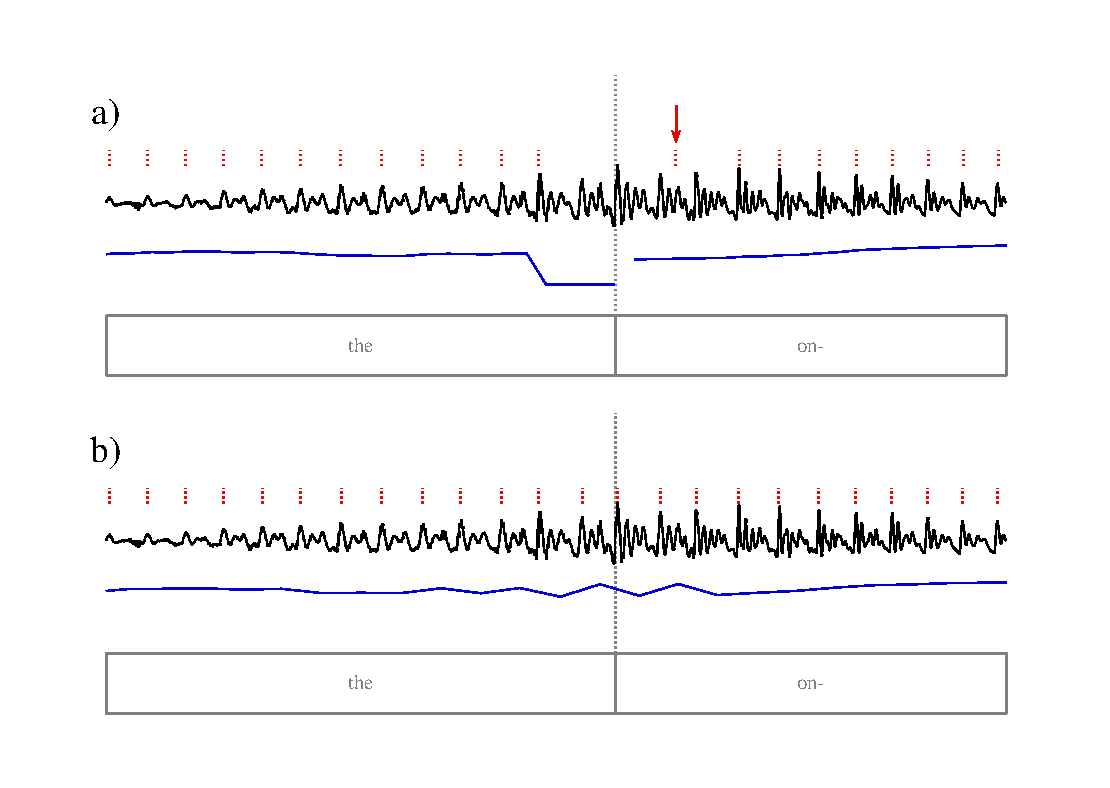
\includegraphics[width=\textwidth,height=0.7\textheight,keepaspectratio]{../figures/creakJitterShimmer/creakJitterShimmer.eps}
%			\caption[Handling of creaky voicing in resynthesis]{Illustration of method for handling creaky\-/voiced portions of speech.  (a)~Excerpt of Talker~\ac{b}’s recording of sentence 33–05, in which vowel hiatus is resolved with light creaky voicing.  The waveform (black) is overlaid with Praat’s auto\-/detected pulse marks (dotted red lines) and pitch track (dashed blue line).  Note the missed cycles on either side of the red arrow, and the phase\-/shift of all pulses right of the arrow.  (b)~The same span of speech after manual correction of pulses, and a (jittery, but continuous) pitch track generated from the corrected pulses.\label{fig:JitShim}}
	\end{itm}
\end{frame}

\begin{frame}{Resynthesis (2 of 3)}
	\begin{itm}
		\item Dynamic time warping of \fo{} and intensity 
		\item[] 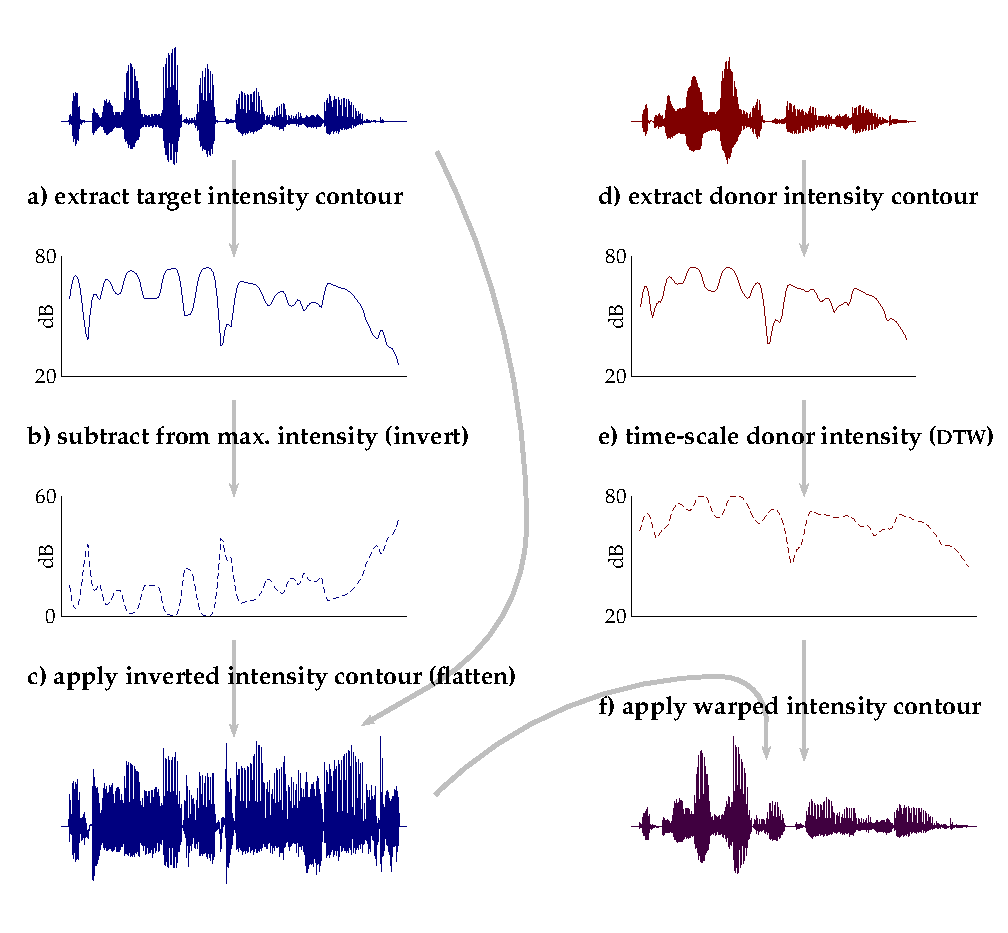
\includegraphics[width=\textwidth,height=0.75\textheight,keepaspectratio]{../figures/intensity/intensity2.eps}
%				\caption[Intensity scaling in resynthesis]{Illustration of the method used to scale intensity.  (a)~Intensity contour is extracted from target waveform (blue).  (b)~The intensity contour of the target signal is inverted, by subtracting each intensity point from the maximum intensity.  (c)~Target intensity is \term{neutralized} or \term{flattened} by multiplying the target signal by the inverted intensity contour.  (d)~Intensity contour is extracted from the prosodic donor signal (red).  (e)~The prosodic donor intensity contour is time\-/scaled syllable\-/by\-/syllable via dynamic time warping (\ac{dtw}) to match the temporal pattern of the target signal.  (f)~The intensity\-/neutralized target signal is multiplied by the time\-/warped donor intensity contour (purple).  The signal is now ready for \psola{} resynthesis of duration and pitch.\label{fig:IntenManip}}
	\end{itm}
\end{frame}

% TODO: next slide: add info that A > B > C

\begin{frame}{Resynthesis (3 of 3)}
	\begin{itm}
		\item \psola{} algorithm as implemented in Praat
		\item[]
		\item \fo, duration \& intensity swapped between all possible pairs of talkers
			\begin{itm}
			\item Nine “talkers” total: \ac{a}, \ac{b}, \ac{c}, \ac{ab}, \ac{ac}, \ac{ba}, \ac{bc}, \ac{ca}, \ac{cb}
			\item[]
			\end{itm}
		\item (Show demo)
%		\item Graphic of how it works?  Demo?
	\end{itm}
\end{frame}

% TODO: next slide not clear
% 90 sentences × (3 unmodified + 6 resynthesized “talkers”) = 810 stimuli
% each listener heard each sentence once (90 total)
% talker-sentence pairings were randomized for each listener

\subsection{Experimental design}
\begin{frame}{Experimental design}
	\begin{itm}
	\item 90 stimuli (9 talkers × 10 sentences each)
		\begin{itm}
		\item Random talker-sentence pairings for each listener
		\item “Repeat what you hear” task, scored by keyword (0–5)
		\item 16 dialect-matched listeners in this exp. (36 total)
		\end{itm}
	\end{itm}
\end{frame}

%===== RESULTS =====%
\section{Results}

\subsection{Behavioral results}
\begin{frame}{Segregating prosodic \& non-prosodic contributions (1 of 2)}
	\begin{itm}
	\item[] Mean keywords correct, ±1 standard error
	\item[] 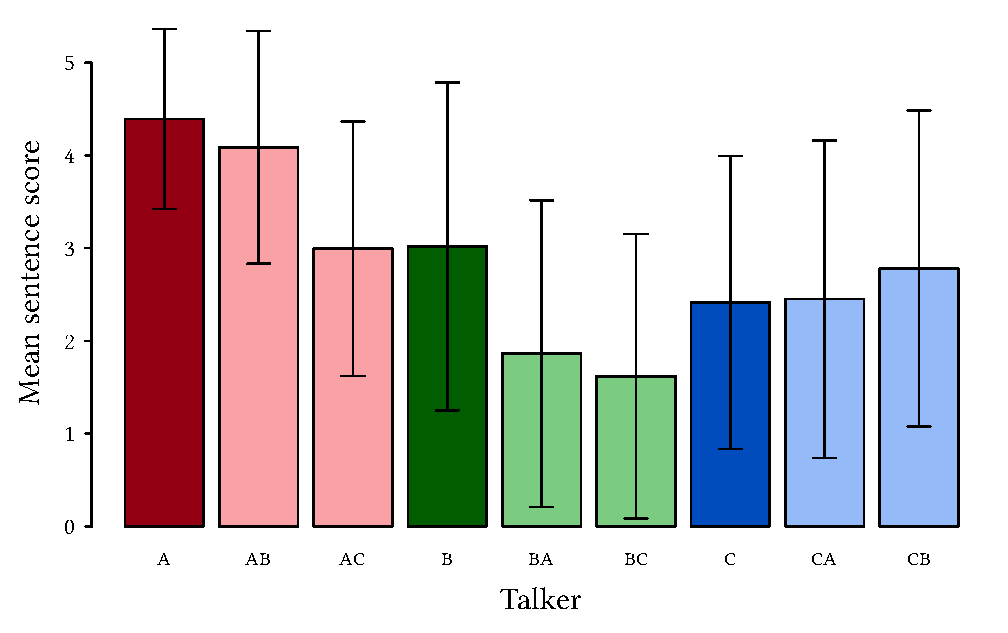
\includegraphics[width=\textwidth,height=0.75\textheight,keepaspectratio]{../figures/results/ExpOneBarplot.eps}
%			\caption[Barplot of mean sentence scores for Experiment~1]{Barplot of mean sentence scores for Experiment~1.  Error bars are ±1 standard error; lighter colors indicate resynthesized talkers, with the second letter indicating the prosodic donor (see Section~\ref{sec:ExpDesign} for full explanation of talker codes).  Similar hues indicate shared segmental donors.\label{fig:ExpOneBarplot}}
	\end{itm}
\end{frame}

\begin{frame}{Segregating prosodic \& non-prosodic contributions (2 of 2)}%
	\begin{columns}[t]
		\begin{column}{0.6\textwidth}
%			\begin{itm}
%			\item[] 
				{\scriptsize
				\begin{tabu}{X[2,m,l] X[1,m,l] X[-1,m,c]}
					\toprule
					\rowfont{\bfseries} \multicolumn{2}{l}{Predictor} & Effect (keywords) \\
					\midrule
								   & {\color{rdd}Talker \ac{a}} & baseline \\
					Prosodic donor & {\color{grn}Talker \ac{b}} & +0.3 \\
								   & {\color{blu}Talker \ac{c}} & −0.6 \\
					\taburulecolor{lgray}\midrule
								   & {\color{rdd}Talker \ac{a}} & baseline \\
					Signal donor   & {\color{grn}Talker \ac{b}} & −1.7 \\
								   & {\color{blu}Talker \ac{c}} & −1.3 \\
					\midrule
					\multicolumn{2}{l}{Resynthesis distortion}                    & −0.7 \\
					\midrule
					\multicolumn{2}{l}{Task familiarization (trial 1 – 90)}       & +0.5 \\
					\midrule
					\multicolumn{2}{l}{Listener variability (standard error)}     & ±0.2 \\
					\midrule
					\multicolumn{2}{l}{Sentence variability (standard error)}     & ±0.7 \\
					\taburulecolor{black}\bottomrule
				\end{tabu}
				}
%			\end{itm}
		\end{column}
		\begin{column}{0.4\textwidth}
%			\begin{itm}
%			\item[] 
			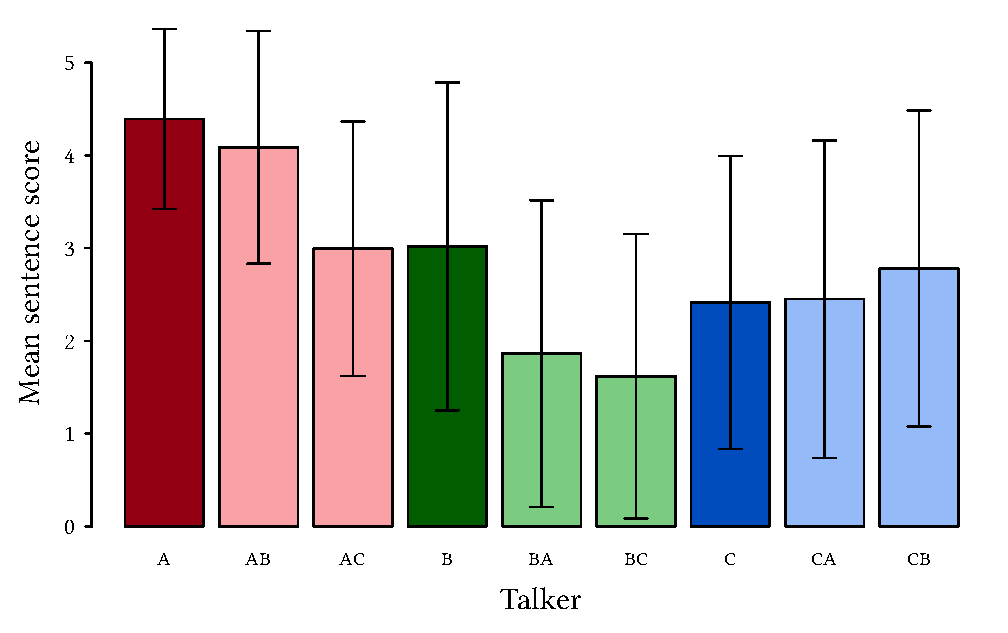
\includegraphics[width=\columnwidth,height=0.75\textheight,keepaspectratio]{../figures/results/ExpOneBarplot.eps}
%			\end{itm}
		\end{column}
	\end{columns}
\end{frame}

%\begin{frame}{Segregating prosodic \& non-prosodic contributions (2 of 2)}%
%	\begin{itm}
%	\item[] 
%		{\small
%		\begin{tabu} spread 3em {X[1,m,l] X[1,m,l] X[-1,m,c]}
%			\toprule
%			\rowfont{\bfseries} \multicolumn{2}{l}{Predictor} & Effect (keywords) \\
%			\midrule
%				           & {\color{rdd}Talker \ac{a}} & baseline \\
%			Prosodic donor & {\color{grn}Talker \ac{b}} & +0.3 \\
%				           & {\color{blu}Talker \ac{c}} & −0.6 \\
%			\taburulecolor{lgray}\midrule
%				           & {\color{rdd}Talker \ac{a}} & baseline \\
%			Signal donor   & {\color{grn}Talker \ac{b}} & −1.7 \\
%				           & {\color{blu}Talker \ac{c}} & −1.3 \\
%			\midrule
%			\multicolumn{2}{l}{Resynthesis distortion}                    & −0.7 \\
%			\midrule
%			\multicolumn{2}{l}{Task familiarization (trial 1 – 90)}       & +0.5 \\
%			\midrule
%			\multicolumn{2}{l}{Listener variability (standard error)}     & ±0.2 \\
%			\midrule
%			\multicolumn{2}{l}{Sentence variability (standard error)}     & ±0.7 \\
%			\taburulecolor{black}\bottomrule
%		\end{tabu}
%		}
%	\end{itm}
%\end{frame}

\subsection{{\itshape Post hoc} acoustic analyses}
\begin{frame}{\Ph{} acoustic analyses (overview)}
	\begin{itm}
	\item[]
	\item[] %{\small
		\begin{tabu} spread 1em {X[m,l] X[-1,m,c]}
			\toprule
			\rowfont{\bfseries} \multicolumn{2}{l}{Patterns seen in the statistical model} \\
			\midrule
			Overall intelligibility & \redd{a} > \grnn{b} > \bluu{c} \\
			\taburulecolor{lgray}\midrule
			Non-prosodic factors    & \redd{a} > \bluu{c} > \grnn{b} \\
			\midrule
			Prosody                 & \grnn{b} > \redd{a} > \bluu{c} \\
			\taburulecolor{black}\bottomrule
		\end{tabu}
%	} %small
	\item[]
	\item<2->[] Which acoustic predictors match those patterns?
		\begin{itm}
		\item<3> Can we segregate predictors tracking \emp{prosodic} contributions to intelligibility from predictors tracking \emp{non-prosodic} contributions to intelligibility? 
		\end{itm}
	\end{itm}
\end{frame}

\begin{frame}{\Ph{} acoustic analyses (overview)}
	\begin{itm}
	\item[] Which acoustic predictors match those patterns?
		\begin{itm}
		\item[]
		\item Overall intelligibility (\redd{a} > \grnn{b} > \bluu{c})
			\begin{itm}
			\item Unreduced stop consonants
			\item Vowel space size: area of polygon based on means
			\item[]
			\end{itm}
		\item<2-> Non-prosodic factors (\redd{a} > \bluu{c} > \grnn{b})
			\begin{itm}
			\item Vowel space size: area of convex hull
			\item Vowel space size: mean distance from center
			\item Vowel space size: F1 range
			\item[]
			\end{itm}
		\item<3> Prosody (\grnn{b} > \redd{a} > \bluu{c})
			\begin{itm}
			\item Nothing matches!
			\end{itm}
		\end{itm}
	\end{itm}
\end{frame}

\begin{frame}{\Ph{} acoustic analyses (prosody)}
	\begin{itm}
	\item[] Relative magnitudes of prosodic metrics
	\item[] 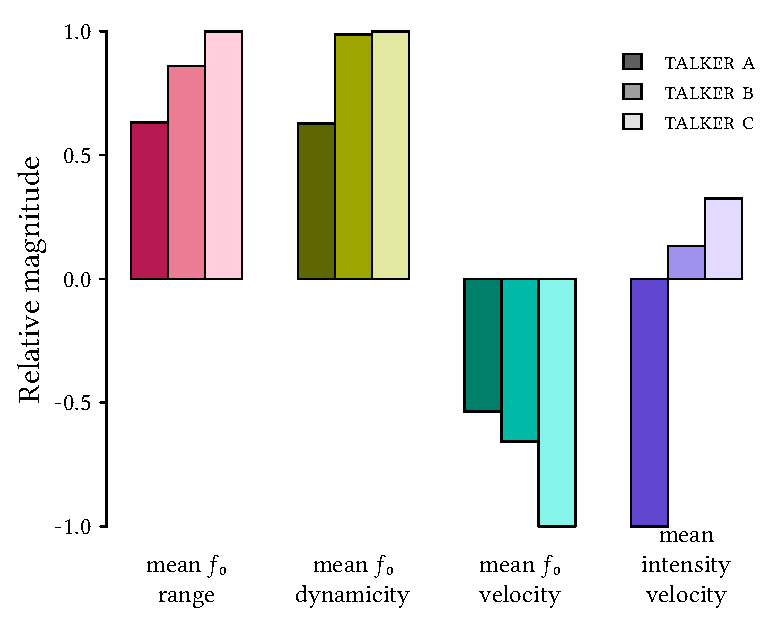
\includegraphics[width=\textwidth,height=0.75\textheight,keepaspectratio]{../figures/posthocs/ProsodicMeasures.eps}
%			\caption[Barplot of prosodic metrics]{Barplot of the relative magnitudes of several prosodic metrics. Each metric has been scaled by dividing by the maximum absolute value among the three talkers.\label{fig:ProsodicMeasures}}
% TODO: separate intensity from pitch (give it its own barplot)
% TODO: add duration if time
% TODO: add vowel space metric barplots?  cluster size?  repulsive force?
	\end{itm}
\end{frame}

\begin{frame}{\Ph{} acoustic analyses (prosody)}
	\begin{columns}[t]
		\begin{column}{0.5\textwidth}
			\begin{itm}
			\item[] 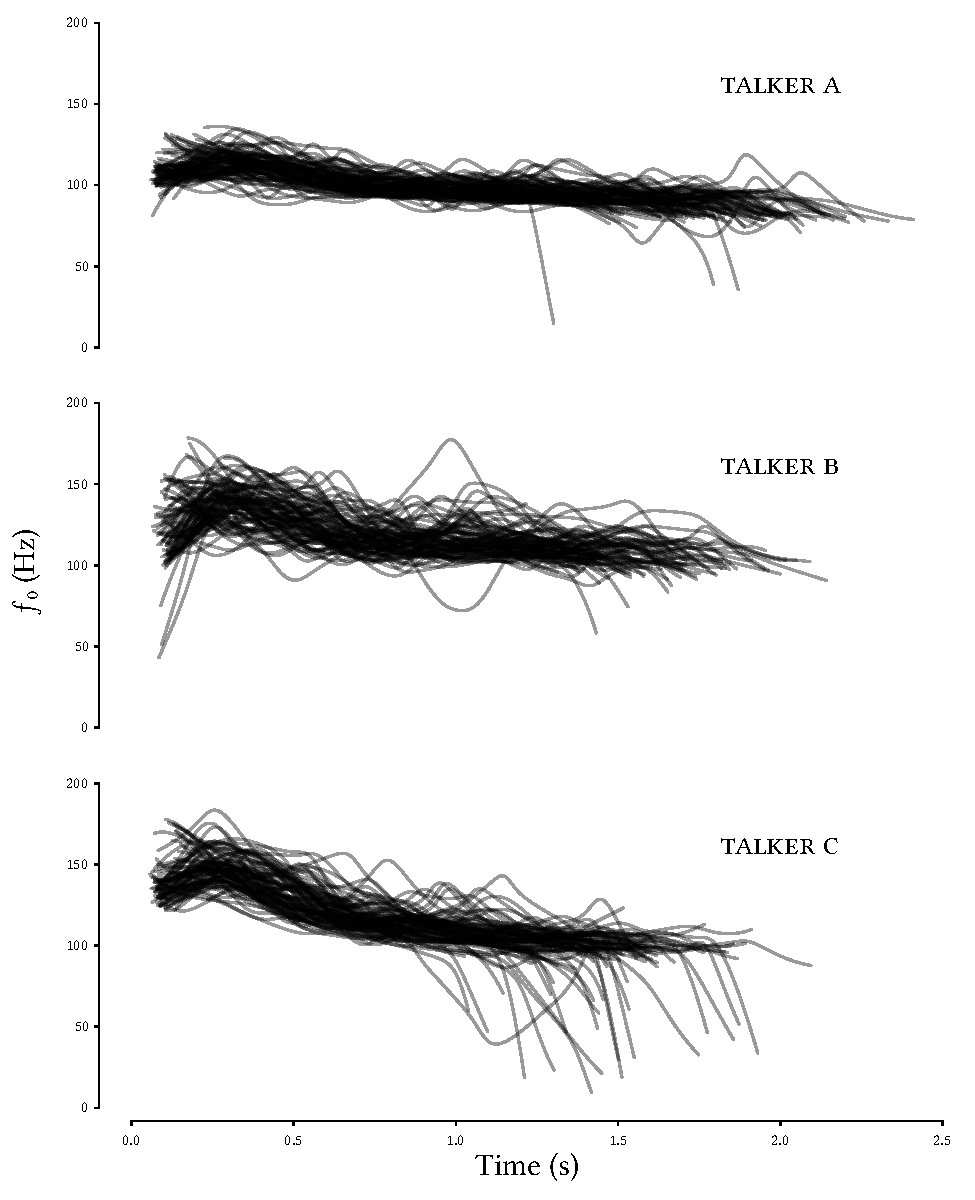
\includegraphics[width=\columnwidth,height=0.75\textheight,keepaspectratio]{../figures/posthocs/PitchTracks.pdf}
					%\caption[Pitch track overlays of the test sentences]{Overlaid pitch tracks for Talkers~\ac{a}, \ac{b} and~\ac{c} for the 90 test sentences.  Pitch tracks have been smoothed by fitting a local polynomial weighted by a Gaussian kernel with a bandwidth of 75 ms.\label{fig:PitchTracks}}
			\end{itm}
		\end{column}
		\begin{column}{0.5\textwidth}
			\begin{itm}
			\item Talker \ac{c}’s creaky voicing inflates \fo~range, dynamicity, \& velocity
				\begin{itm}
				\item[]
				\end{itm}
			\item<2> If we ignore \bluu{c}, prosody predicts \grnn{b}~>~\redd{a}.  Matches:
				\begin{itm}
				\item Mean \fo{} range
				\item Mean \fo{} dynamicity
				\end{itm}
			\end{itm}
		\end{column}
	\end{columns}
\end{frame}

\begin{frame}{\Ph{} acoustic analyses (prosody)}
	\begin{itm}
	\item[] Relative magnitudes of prosodic metrics
	\item[] 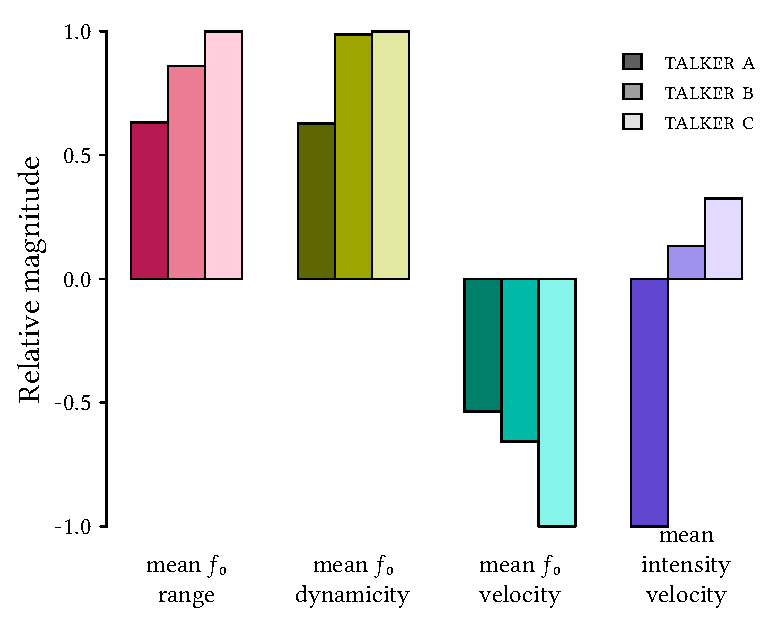
\includegraphics[width=\textwidth,height=0.75\textheight,keepaspectratio]{../figures/posthocs/ProsodicMeasures.eps}
%			\caption[Barplot of prosodic metrics]{Barplot of the relative magnitudes of several prosodic metrics. Each metric has been scaled by dividing by the maximum absolute value among the three talkers.\label{fig:ProsodicMeasures}}
	\end{itm}
\end{frame}

\begin{frame}{\Ph{} acoustic analyses (intensity)}
	\begin{columns}[t]
		\begin{column}{0.5\textwidth}
			\begin{itm}
			\item[] 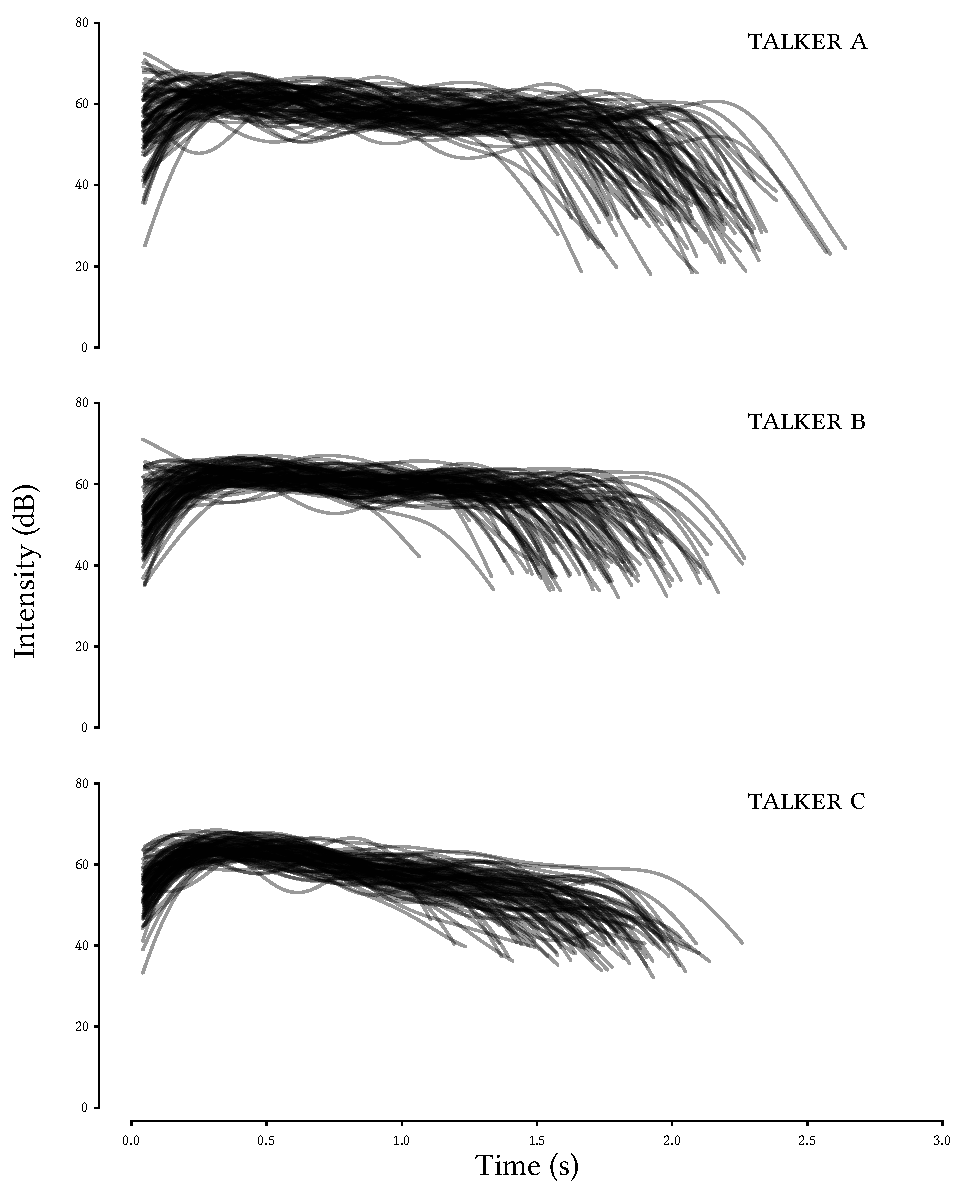
\includegraphics[width=\columnwidth,height=0.75\textheight,keepaspectratio]{../figures/posthocs/IntensityTracks.pdf}
					%\caption[Pitch track overlays of the test sentences]{Overlaid pitch tracks for Talkers~\ac{a}, \ac{b} and~\ac{c} for the 90 test sentences.  Pitch tracks have been smoothed by fitting a local polynomial weighted by a Gaussian kernel with a bandwidth of 75 ms.\label{fig:PitchTracks}}
			\end{itm}
		\end{column}
		\begin{column}{0.5\textwidth}
			\begin{itm}
			\item Talker \ac{a}’s utterance-final downtrend dominates
				\begin{itm}
				\item[]
				\end{itm}
			\item Talker \ac{c}’s more gradual downtrend (higher mean intensity velocity) may actually decrease intelligibility by compromising word-level \ac{snr}
				\begin{itm}
				\item[]
				\end{itm}
			\item More research needed
			\end{itm}
		\end{column}
	\end{columns}
\end{frame}


%===== DISCUSSION =====%
\section{Discussion}

\begin{frame}{Discussion}
	\begin{itm}
	\item[] Why does area of \emp{vowel means} polygon follow overall intelligibility pattern (\redd{a} > \grnn{b} > \bluu{c}), but area of \emp{convex hull} follows non-prosodic pattern (\redd{a} > \bluu{c} > \grnn{b})? 
		\begin{itm}
		\item[]
		\item<2-> Formant values are from lexically stressed vowels in keywords \emp{throughout sentence}
		\item[]
		\item<3-> Thus variation in F1 \& F2 reflects low-level variation (coarticulation) and variation due to prosody (phrasal accent)
		\item[]
		\item<4> \emp{Mean} formant values reflect this variation; convex hull indexes only \emp{extreme} values
		\end{itm}
	\end{itm}
\end{frame}

\begin{frame}{Things I could say a lot more about...}
	\begin{itm}
	\item<1,2> Why does \# of release bursts follow  overall intelligibility pattern instead of non-prosodic pattern?
		\begin{itm}
		\only<2>{%
		\item Prosody affects prominence, and prominence (partially) determines stop articulation.  Speech rate, phrasal stress, domain-initial strengthening may all play a role.
		}
		\item[]
		\end{itm}
	\item<1,3> About those keywords... 
		\begin{itm}
		\only<3>{%
		\item No good scoring method exists.  Some keywords easier than others.  We can model this to some extent, but there are still “near miss” \vs\ “totally wrong” responses; this is not captured by counting 1’s and 0’s.
		}
		\item[]
		\end{itm}
	\item<1,4> What about familiarity?
		\begin{itm}
		\only<4>{%
		\item I really wanted to find out what underlies the familiar talker advantage.  Unfortunately experiment 2 didn’t work.  Listeners showed differential accommodation to different training talkers, but did not retain the advantage into the testing phase (when talkers were presented randomly).  More research needed.
		}
		\item[]
		\end{itm}
	\end{itm}
\end{frame}

%===== REFERENCES =====%
% Don't give this its own section, unless you want an auto-generated return to the outline slide just before it
\begin{frame}{References}
	\tiny
	\bibliography{../dissertation}
	\bibliographystyle{../apa-custom}
\end{frame}


%\subsection{Acknowledgments} % include if you want on the outline / in PDF bookmarks
\begin{frame}{Acknowledgments}
	\begin{itm}
		\centering
		\item[] Thanks to:
		\item[] 
		\item[] Richard~Wright, Sharon~Hargus, Gina-Anne~Levow,\\Erick~Gallun, Pam~Souza
		\item[] 
		\item[] Jennifer~Haywood, Gus~McGrath, Steve~Moran, Darren~Tanner,\\members~of~the~UW~Phonetics~Lab
		\item[] 
		\item[] Sherry~Brown, David~Adams, Dennis~Lamb, Bill~Moody,\\Larry~BonJour, Bill~Talbott, David~Knechteges, Bi~Nyan-Ping,\\Zev~Handel, Chris~Stecker, KC~Lee
		\item[] 
		\item[] Sarala~Puthuval
	\end{itm}
\end{frame}

%\begin{frame}{Segregating prosodic \& non-prosodic contributions (2 of 2)}
%	Statistical model: Fixed effects\\ \vspace{\baselineskip}
%	{\small
%	\begin{tabu} spread 1.5em {Xrcr >{\hl}l}
%		\toprule
%		\multicolumn{5}{l}{Summary of fixed effects (N=1440; log-likelihood=−2551)}\\
%		\rowfont\bfseries
%		\multicolumn{1}{l}{Predictor} & \multicolumn{1}{c}{Coefficient} & \textit{s} & \multicolumn{1}{c}{\itshape t} & \multicolumn{1}{c}{\itshape p}\\
%		\midrule
%		Intercept           &  4.132 & (0.145) &  28.44 & <10⁻¹⁶\\
%		resynth = \ac{true} & −0.662 & (0.077) &  −8.63 & <10⁻¹⁶\\
%		segDonor = \ac{b}   & −1.673 & (0.089) & −18.86 & <10⁻¹⁶\\
%		segDonor = \ac{c}   & −1.278 & (0.089) & −14.31 & <10⁻¹⁶\\
%		proDonor = \ac{b}   &  0.307 & (0.088) &   3.48 & <10⁻³\\
%		proDonor = \ac{c}   & −0.646 & (0.088) &  −7.36 & <10⁻¹²\\
%%		\rowfont{\color{frametitle.fg}}
%		trial               &  0.006 & (0.001) &   4.02 & <10⁻⁴\\
%		\bottomrule
%	\end{tabu}
%	}
%\end{frame}

\end{document}
